\documentclass{article}
\usepackage[utf8]{inputenc}
\usepackage[brazilian]{babel}
\usepackage{graphicx}
\usepackage{float}
\usepackage[pdftex]{hyperref}
\usepackage{epstopdf}
\usepackage{etoolbox}
\usepackage{amsmath}
\usepackage{amsfonts}
\usepackage{amssymb}
\usepackage{caption}
\usepackage{subcaption}
\usepackage{setspace}
\usepackage{tikz}

\patchcmd{\thebibliography}{\section*}{\section}{}{}
\newcommand{\R}{\ensuremath{\mathbb{R}}}
\newcommand{\Prob}{\ensuremath{\mathbb{P}}}
\newcommand{\K}{\ensuremath{\mathbb{K}}}
\newcommand{\U}{\ensuremath{\mathbb{U}}}
\newcommand{\N}{\ensuremath{\mathbb{N}}}
\newcommand{\Lg}{\ensuremath{\mathbb{L}}}
\newcommand{\T}{\ensuremath{\rm Tr}}
\newcommand{\sg}{{\sigma(x_k)}}

\newcommand{\G}{\ensuremath{\mathcal{G}}}
\newcommand{\F}{\ensuremath{\mathcal{F}}}
\newcommand{\C}{\ensuremath{\mathcal{C}}}
\newcommand{\E}{\ensuremath{\mathcal{E}}}
\newcommand{\Hn}{\ensuremath{\mathcal{H}}}
%\newcommand{\Hoo}{\ensuremath{\mathcal{H}_\infty}}
\newcommand{\Hop}{\ensuremath{\mathcal{H}_{op}}}
% --------------------------------------------------
\newtheorem{theo}{Teorema}
\newtheorem{exa}{Exemplo}
\newtheorem{lemm}{Lema}
\newtheorem{coro}{Corolário}
\newtheorem{defn}{Definição}[section]

%opening


\begin{document}

\begin{titlepage}
\begin{center}

\newcommand{\HRule}{\rule{\linewidth}{0.5mm}}
% Upper part of the page. The '~' is needed because \\
% only works if a paragraph has started.

\includegraphics[width=0.15\textwidth]{logoUnicamp}~\\[1cm]

\textsc{\LARGE Universidade Estadual de Campinas}\\[1.5cm]

\textsc{\Large Faculdade de Engenharia Mecânica}\\[0.5cm]

% Title
\HRule \\[0.4cm]
{ \huge \bfseries ES827 - Robótica Industrial\\ \vspace{1cm} Projeto Final \\
\Large{Dinâmica e Cinemática do Robô Puma 560} \\[0.4cm] }

\HRule \\[1.5cm]

% Author and supervisor
\begin{minipage}{0.6\textwidth}
\begin{flushleft} \large
\emph{Nome:}\\
Daniel Dello Russo Oliveira\\ Marcelli Tiemi Kian
\end{flushleft}
\end{minipage}
\begin{minipage}{0.2\textwidth}
\begin{flushright} \large
\emph{RA}\\ 101918\\
117892
\end{flushright}
\end{minipage}

\vfill

% Bottom of the page
{\large \today}

\end{center}
\end{titlepage}


\onehalfspacing
\section{Objetivos} 
O objetivo desse projeto é simular e analisar aspectos dinâmicos de um robô Puma 560, e cinemática de um robô criado pelo arquivo ``ini\_Rbt.m"\cite{bb:inirbt} conforme sugerido pelo roteiro\cite{bb:roteiro}. 
	
\section{Dinâmica do Puma 560}
Pelo roteiro foi sugerido para a análise dinâmica, utilizar o robô Puma 560 construído automaticamente pela ``toolbox" de robótica\cite{bb:toolbox}, a função ``accel" e a ``Matlab Function" pelo Simulink. Entretanto, algumas modificações foram feitas. Retiramos o atrito seco (de Coulomb) nas juntas do robô, pois gerava longos tempos de simulação, e utilizamos um ``script" do Matlab em vez de usar o Simulink.

\subsection{Malha aberta}
A seção 6.3 da tese\cite{bb:tese} utilizada como base mostra simulações feitas com o robô em malha aberta. A partir de entradas desejadas para $q_{des}$ e $\dot{q_{des}}$ calculamos o vetor de torque $u$ necessário para manter a posição. Como podemos observar, fizemos as simulações abaixo utilizando o robô Puma 560 também em malha aberta para as mesmas condições iniciais informadas pela tese\cite{bb:tese}, mas com o vetor $u$ calculado para o robô Puma 560.

\begin{equation}
\label{eq:qdesejado}
q_{des}=\begin{bmatrix}
0 & \frac{\pi}{2} & -\frac{\pi}{2} & 0 & 0 & 0
\end{bmatrix}^T
\end{equation}

\begin{equation}
\label{eq:qddesejado}
\dot{q_{des}}=\begin{bmatrix}
0 & 0 & 0 & 0 & 0 & 0
\end{bmatrix}^T
\end{equation}

\begin{equation}
\label{eq:torques}
u=\begin{bmatrix}
0 & -0.7752 & 0.2489 & 0 & 0 & 0
\end{bmatrix}^T
\end{equation}

\subsubsection{Simulação 1}
Condições iniciais:
\begin{equation}
\label{eq:sim1q}
q_{init}=\begin{bmatrix}
0 & 0 & 0 & 0 & 0 & 0
\end{bmatrix}^T
\end{equation}
\begin{equation}
\label{eq:sim1qd}
\dot{q_{init}}=\begin{bmatrix}
0 & 0 & 0 & 0 & 0 & 0
\end{bmatrix}^T
\end{equation}

\begin{figure}[H]
	\centering
	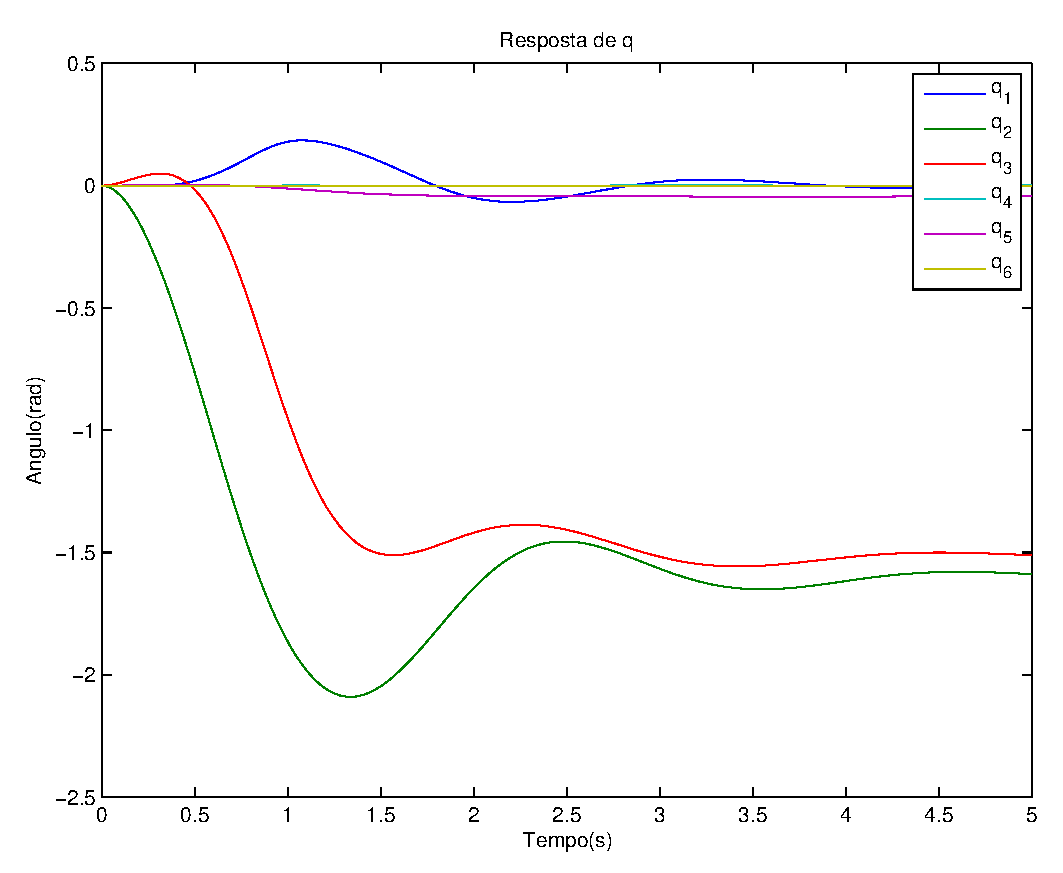
\includegraphics[width=0.8\linewidth]{../sim1ode}
	\caption{Simulação 1 para o robô Puma}
	\label{fig:pumasim1}
\end{figure}

\subsubsection{Simulação 2}
Condições iniciais:
\begin{equation}
\label{eq:sim2q}
q_{init}=\begin{bmatrix}
0 & \pi & -\frac{\pi}{2} & 0 & 0 & 0
\end{bmatrix}^T
\end{equation}
\begin{equation}
\label{eq:sim2qd}
\dot{q_{init}}=\begin{bmatrix}
0 & 0 & 0 & 0 & 0 & 0
\end{bmatrix}^T
\end{equation}

\begin{figure}[H]
	\centering
	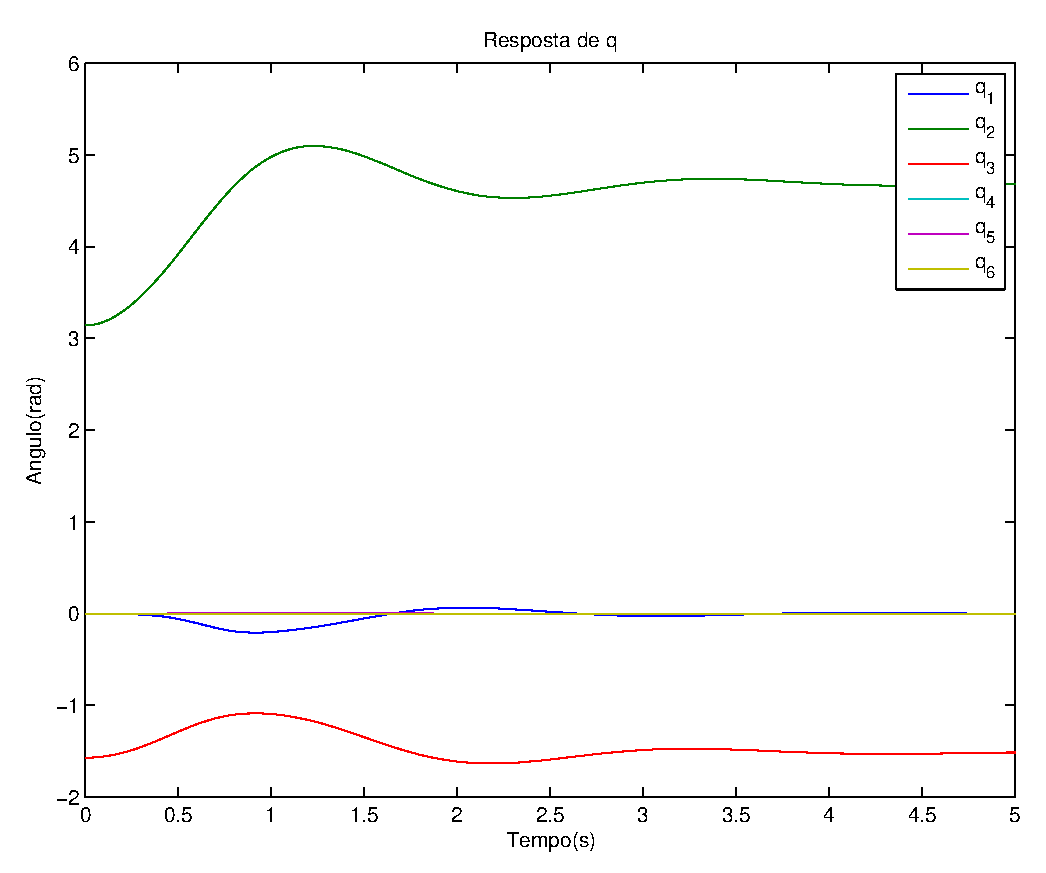
\includegraphics[width=0.8\linewidth]{../sim2ode}
	\caption{Simulação 2 para o robô Puma}
	\label{fig:pumasim2}
\end{figure}

\subsubsection{Simulação 3}
Condições iniciais:
\begin{equation}
\label{eq:sim3q}
q_{init}=\begin{bmatrix}
0 & \frac{\pi}{2} & -\frac{\pi}{2} & 0 & 0 & 0
\end{bmatrix}^T
\end{equation}
\begin{equation}
\label{eq:sim3qd}
\dot{q_{init}}=\begin{bmatrix}
0 & 0 & 0 & 0 & 0 & 0
\end{bmatrix}^T
\end{equation}

\begin{figure}[H]
	\centering
	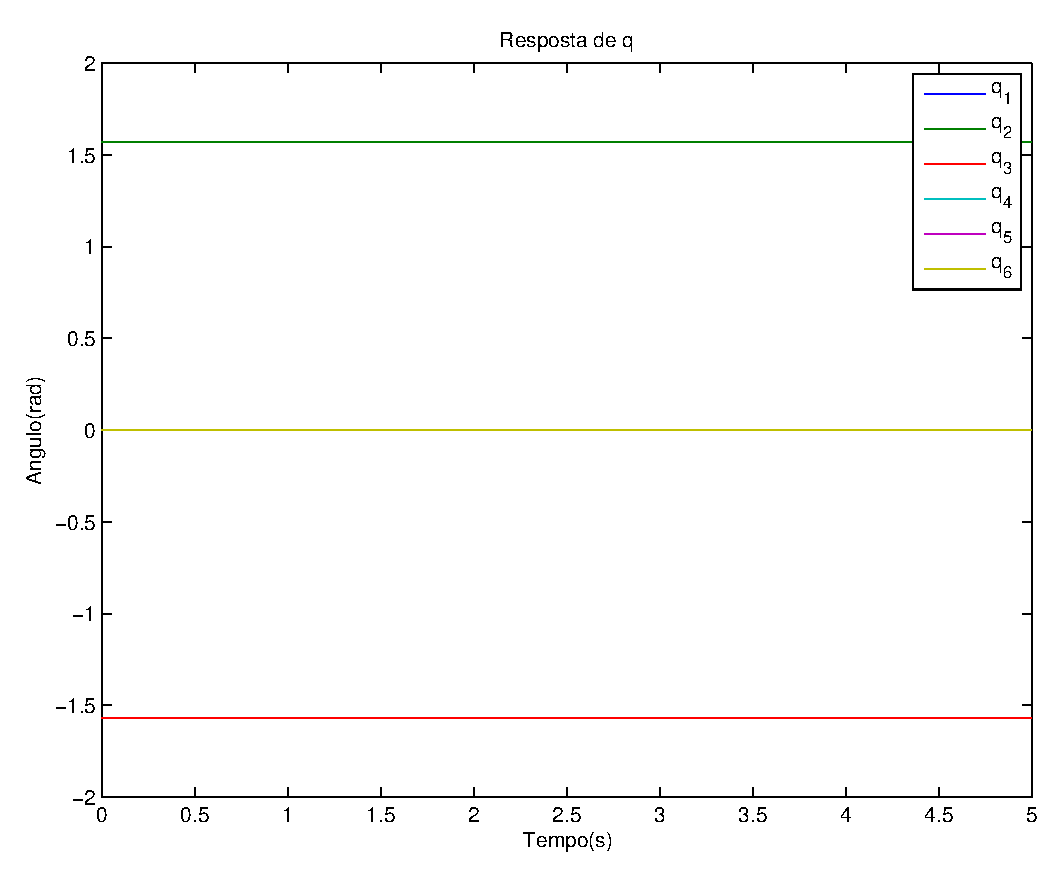
\includegraphics[width=0.8\linewidth]{../sim3ode}
	\caption{Simulação 3 para o robô Puma}
	\label{fig:pumasim3}
\end{figure}

\subsubsection{Simulação 4}
Condições iniciais:
\begin{equation}
\label{eq:sim4q}
q_{init}=\begin{bmatrix}
0 & \frac{\pi}{2}+0.05 & -\frac{\pi}{2} & 0 & 0 & 0
\end{bmatrix}^T
\end{equation}
\begin{equation}
\label{eq:sim4qd}
\dot{q_{init}}=\begin{bmatrix}
0 & 0 & 0 & 0 & 0 & 0
\end{bmatrix}^T
\end{equation}

\begin{figure}[H]
	\centering
	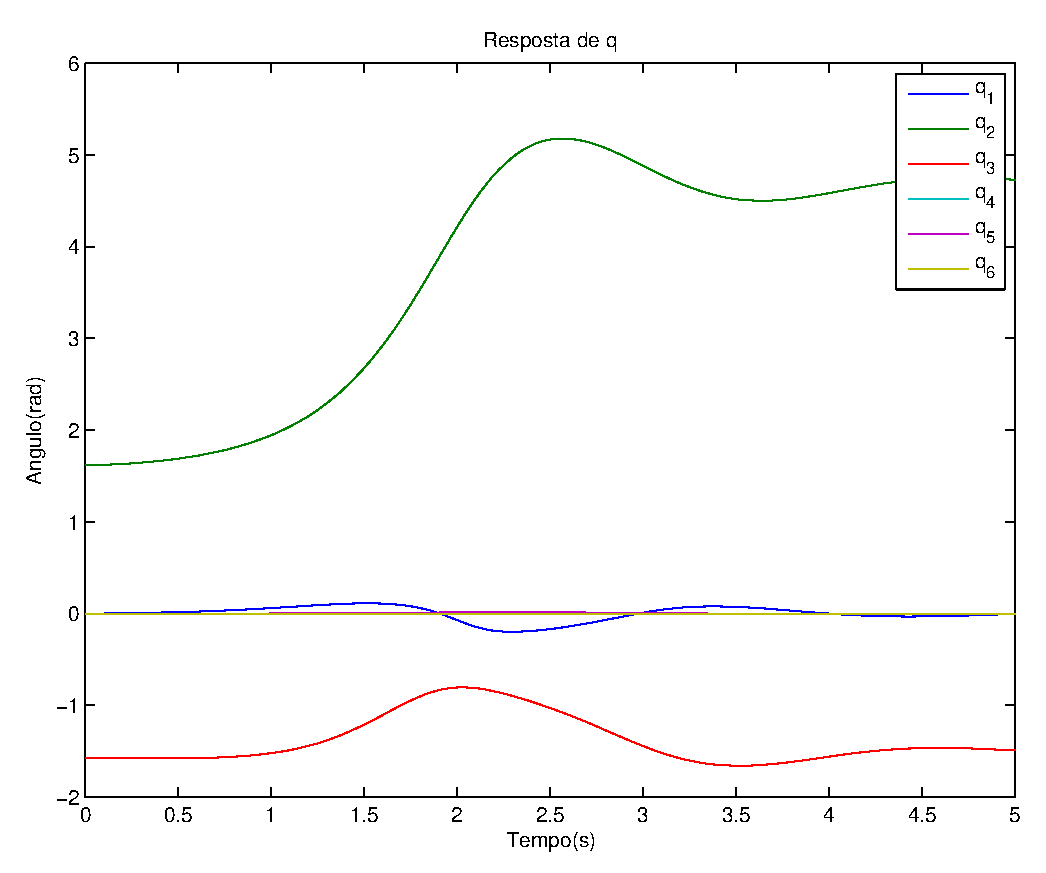
\includegraphics[width=0.8\linewidth]{../sim4ode}
	\caption{Simulação 4 para o robô Puma}
	\label{fig:pumasim4}
\end{figure}

Conforme podemos observar, controlar o sistema em malha aberta colocando como entrada o torque necessário $u$ para manter o robô em uma determinada posição e velocidade $q_{des}$ e $\dot{q_{des}}$ não é sempre possível. Nas simulações feitas acima, apenas a simulação 3 na figura \ref{fig:pumasim3} que possui condições iniciais de posição e velocidade iguais às condições desejadas consegue se manter na posição, pois o torque aplicado foi calculado especificamente para isso. 

Nas demais simulações podemos verificar o torque é insuficiente para levar o robô para a posição desejada, e este acaba indo para uma posição de equilíbrio de menor energia potencial, como pode-se observar pelos valores finais de $q_2$ nas figuras \ref{fig:pumasim1}, \ref{fig:pumasim2} e \ref{fig:pumasim4}. Ainda na figura \ref{fig:pumasim4}, podemos ver que mesmo uma pequena diferença entre a condição inicial e a desejada fazem com que o robô não atinja a posição desejada.

Isto acontece porque as entradas do sistema em malha aberta não dependem de suas saídas, ou seja, não há realimentação. Para o robô se deslocar de sua  posição inicial até a posição desejada são necessários um conjunto de torques sucessivos que variam de acordo com o posicionamento intermediário do robô. No entanto, em malha aberta não temos esta informação sobre a posição intermediária do robô, e aplicamos somente o torque necessário para manter o robô em equilíbrio quando ele já está em sua posição desejada.

\subsection{Equilíbrio de energia}
A seção 6.4 da tese\cite{bb:tese} utilizada como base trata da análise de equilíbrio de energia do robô. No nosso estudo, vamos considerar nulos os esforços de compensação da força gravitacional, fazendo um estudo da energia cinética do robô Puma 560 (translação e rotação), conforme mostrado nas simulações a seguir, sendo as simulações 5 e 6 feitas com atrito viscoso (sem atrito seco), e sem atrito viscoso nem atrito seco.

\subsubsection{Simulação 5}
Condições iniciais e torque:
\begin{equation}
\label{eq:sim5q}
q_{init}=\begin{bmatrix}
0 & 0 & 0 & 0 & 0 & 0
\end{bmatrix}^T
\end{equation}
\begin{equation}
\label{eq:sim5qd}
\dot{q_{init}}=\begin{bmatrix}
0 & 0 & 0 & 0 & 0 & 0
\end{bmatrix}^T
\end{equation}
\begin{equation}
\label{eq:sim5tau}
\tau=\begin{bmatrix}
0 & 0 & 0 & 0 & 0 & 0
\end{bmatrix}^T
\end{equation}

\begin{figure}[H]
	\centering
	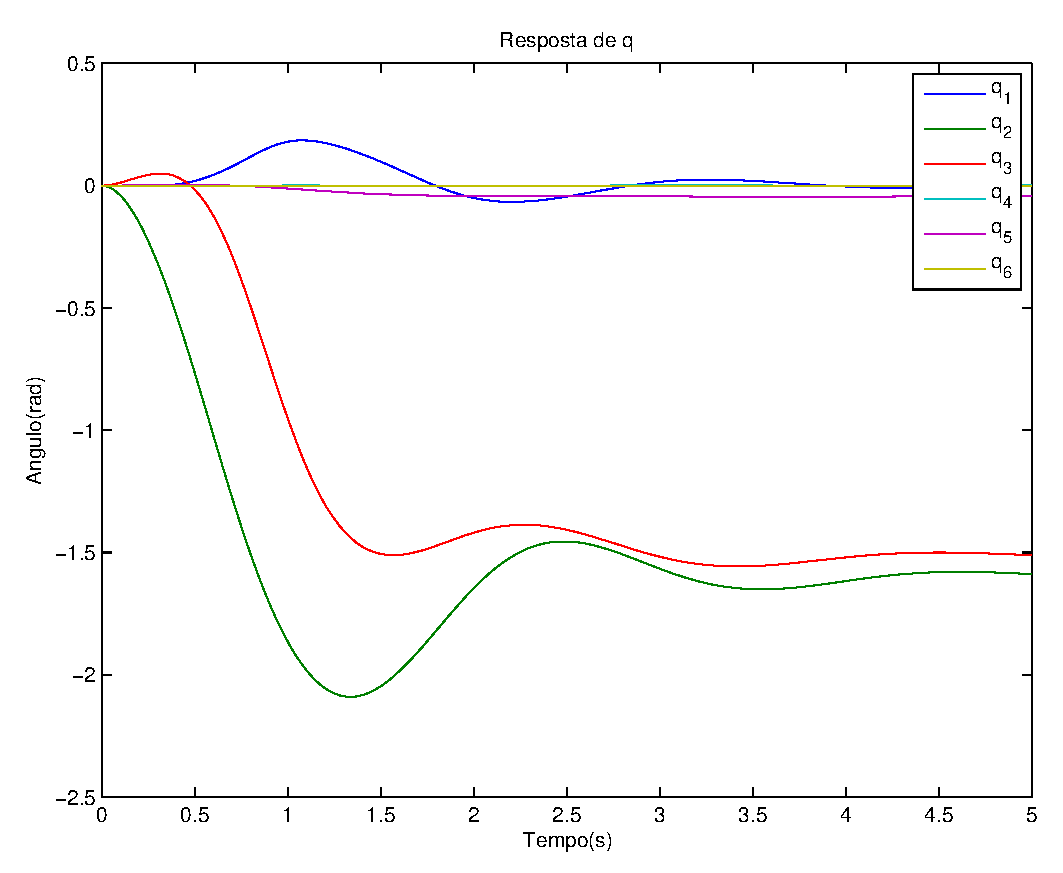
\includegraphics[width=0.8\linewidth]{../sime1odea}
	\caption{Simulação 5 para o robô Puma com atrito viscoso}
	\label{fig:pumasim5}
\end{figure}

\begin{figure}[H]
	\centering
	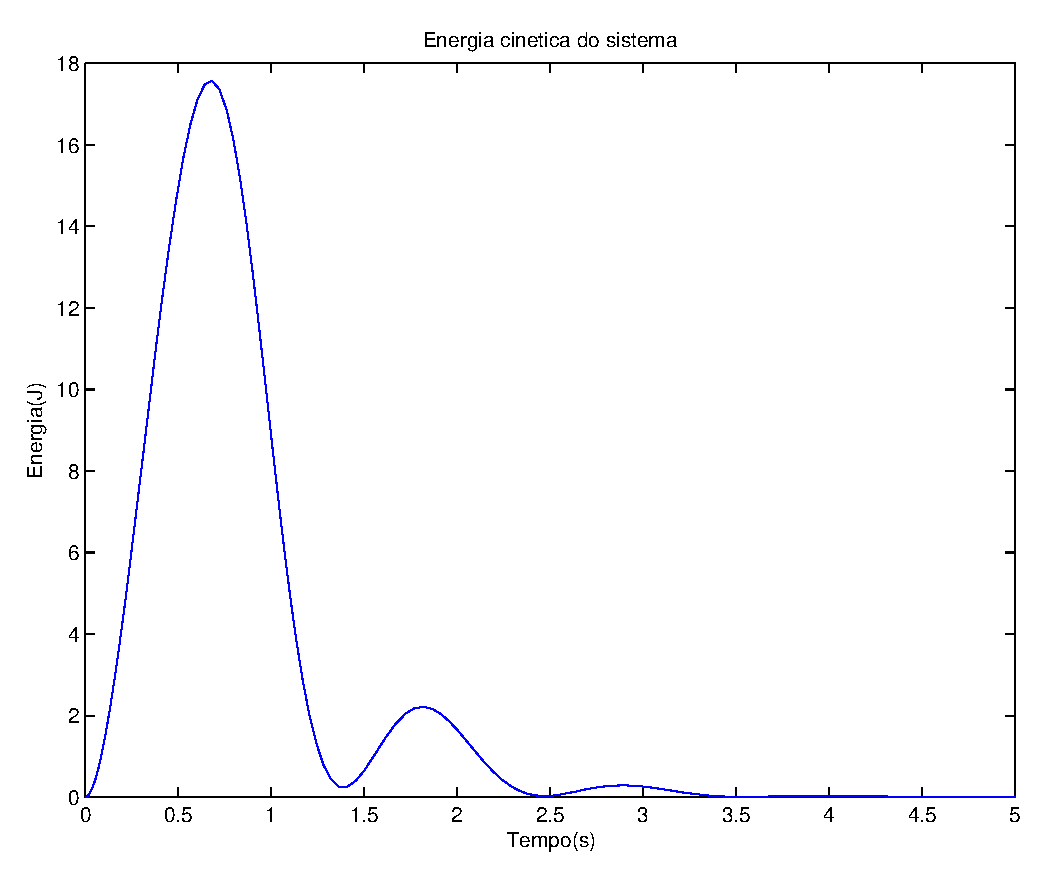
\includegraphics[width=0.8\linewidth]{../sime1kina}
	\caption{Simulação 5 para energia do robô Puma com atrito viscoso}
	\label{fig:energysim5}
\end{figure}

\begin{figure}[H]
	\centering
	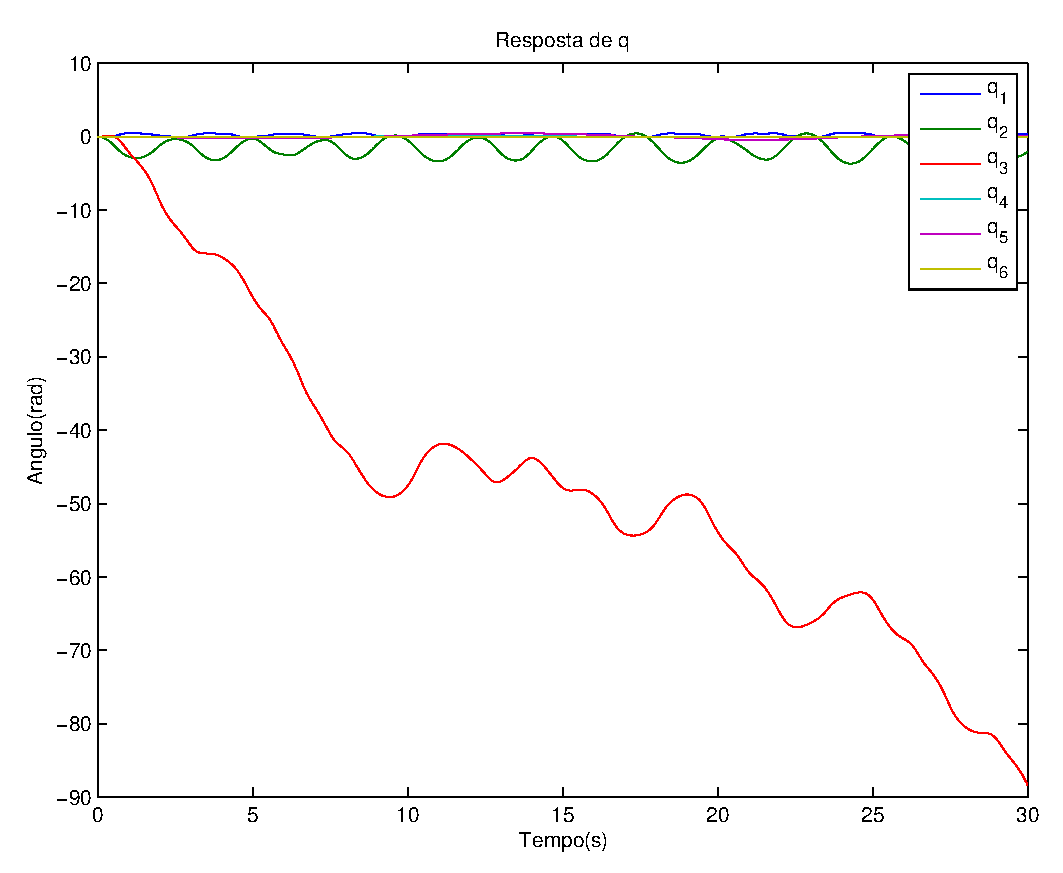
\includegraphics[width=0.8\linewidth]{../longsims/sime1ode.eps}
	\caption{Simulação 5 para o robô Puma sem atrito viscoso}
	\label{fig:pumasim5nf}
\end{figure}

\begin{figure}[H]
	\centering
	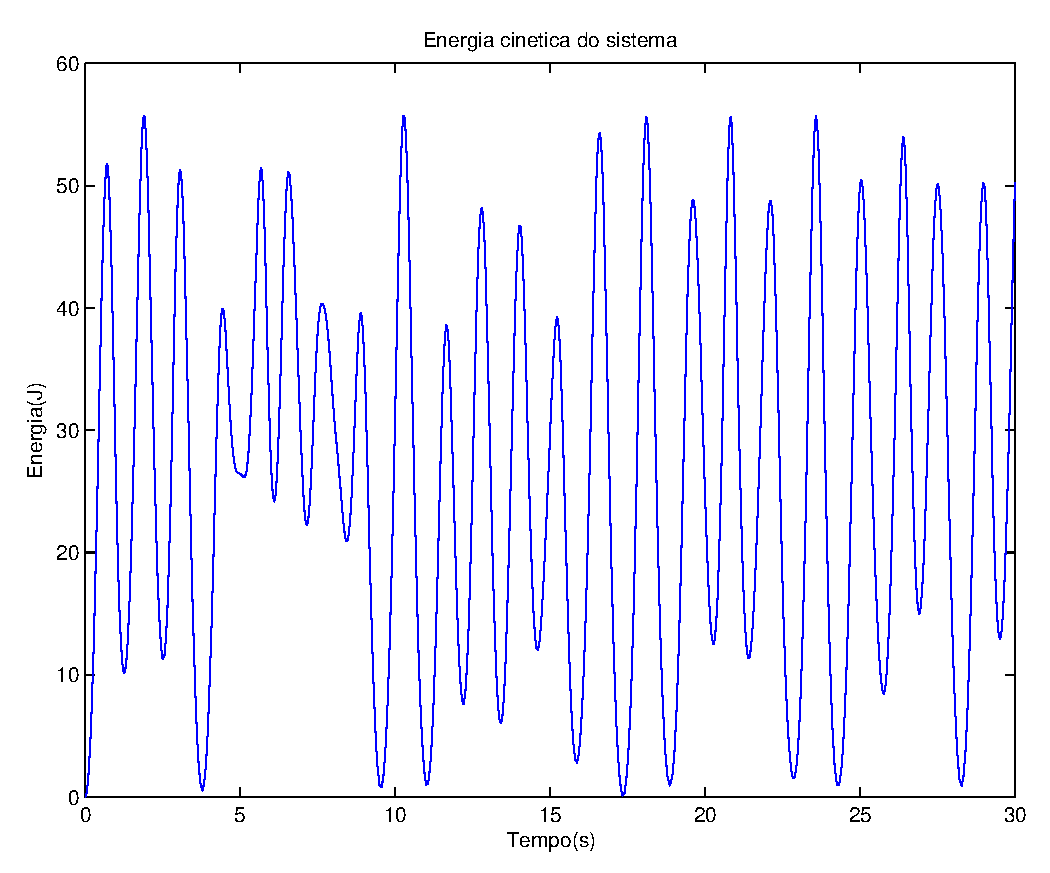
\includegraphics[width=0.8\linewidth]{../longsims/sime1kin.eps}
	\caption{Simulação 5 para energia do robô Puma sem atrito viscoso}
	\label{fig:energysim5nf}
\end{figure}

\subsubsection{Simulação 6}
Condições iniciais e torque:
\begin{equation}
\label{eq:sim6q}
q_{init}=\begin{bmatrix}
0 & 0.000001 & 0 & 0 & 0 & 0
\end{bmatrix}^T
\end{equation}
\begin{equation}
\label{eq:sim6qd}
\dot{q_{init}}=\begin{bmatrix}
0 & 0 & 0 & 0 & 0 & 0
\end{bmatrix}^T
\end{equation}
\begin{equation}
\label{eq:sim6tau}
\tau=\begin{bmatrix}
0 & 0 & 0 & 0 & 0 & 0
\end{bmatrix}^T
\end{equation}

\begin{figure}[H]
	\centering
	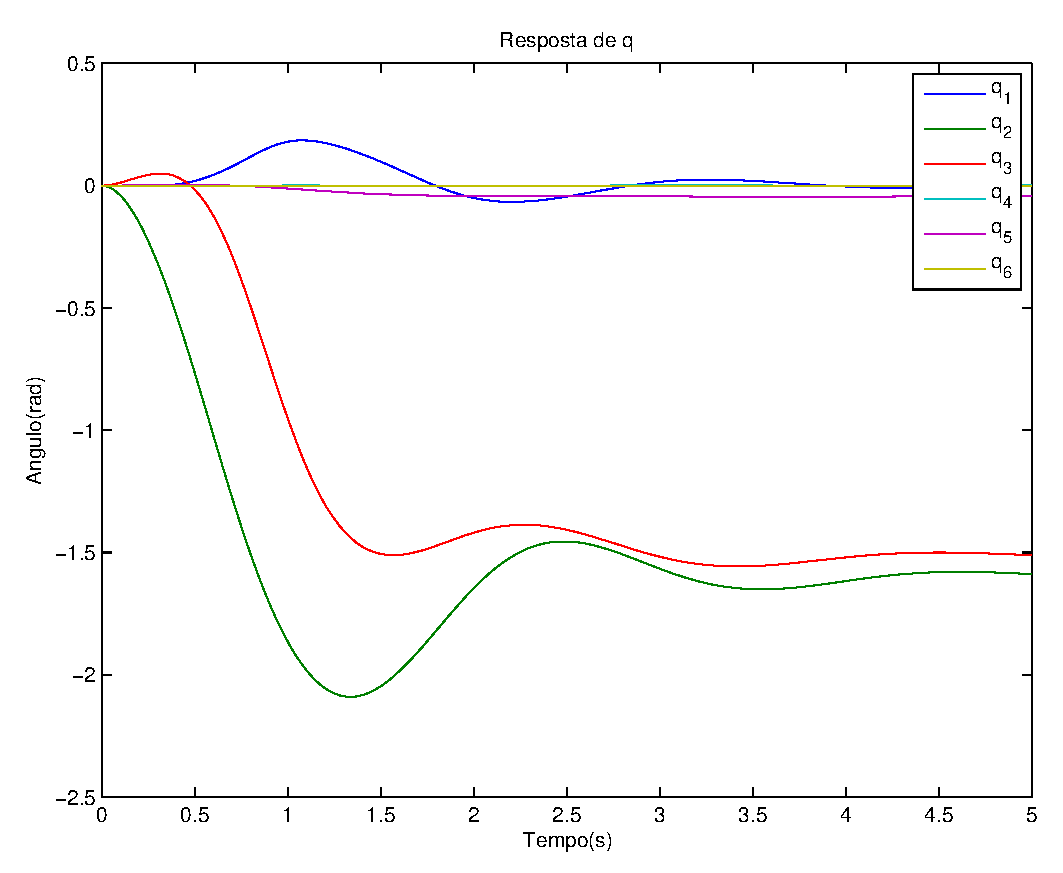
\includegraphics[width=0.8\linewidth]{../sime2odea}
	\caption{Simulação 6 para o robô Puma com atrito viscoso}
	\label{fig:pumasim6}
\end{figure}

\begin{figure}[H]
	\centering
	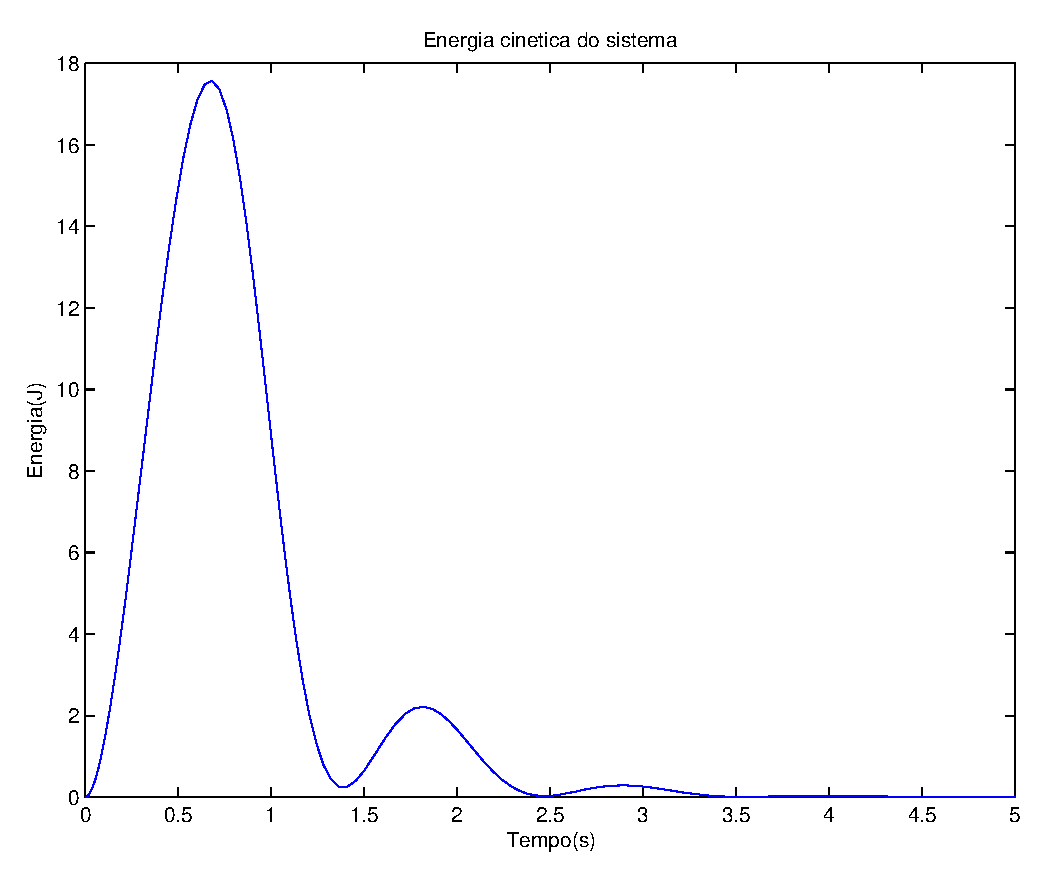
\includegraphics[width=0.8\linewidth]{../sime1kina}
	\caption{Simulação 6 para energia o robô Puma com atrito viscoso}
	\label{fig:energysim6}
\end{figure}

\begin{figure}[H]
	\centering
	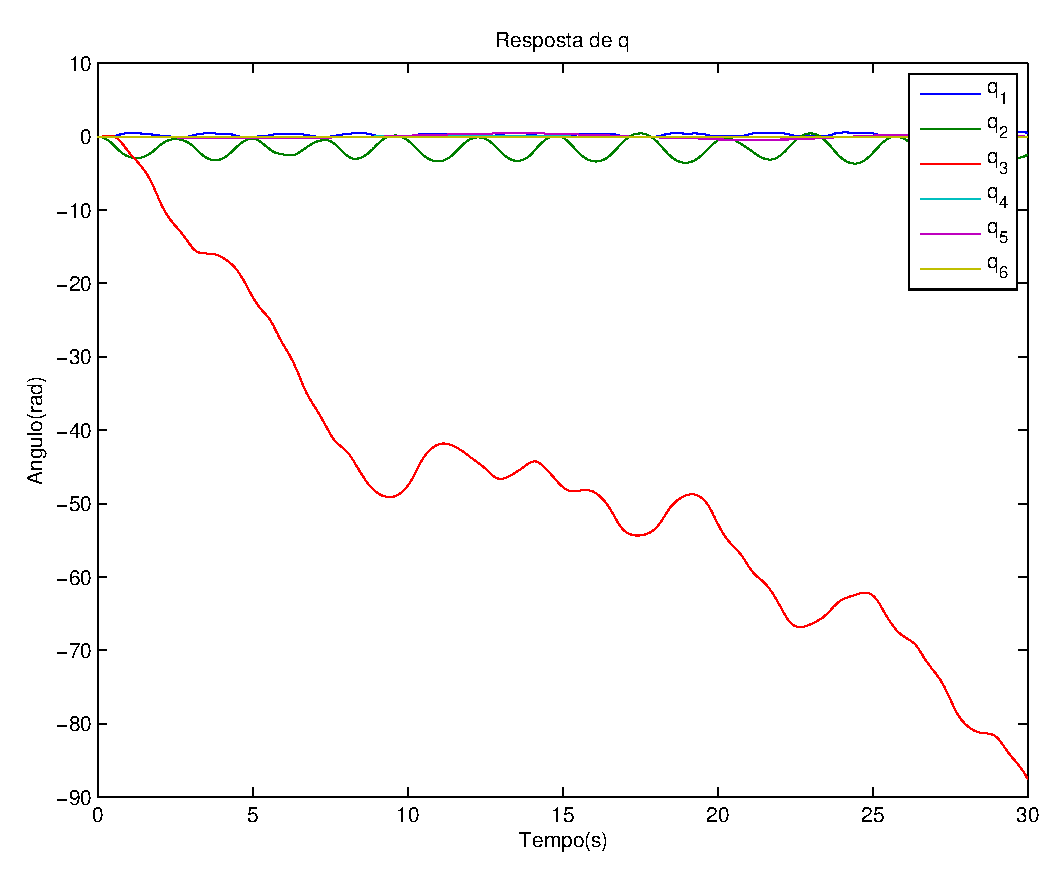
\includegraphics[width=0.8\linewidth]{../longsims/sime2ode.eps}
	\caption{Simulação 6 para o robô Puma sem atrito viscoso}
	\label{fig:pumasim6nf}
\end{figure}

\begin{figure}[H]
	\centering
	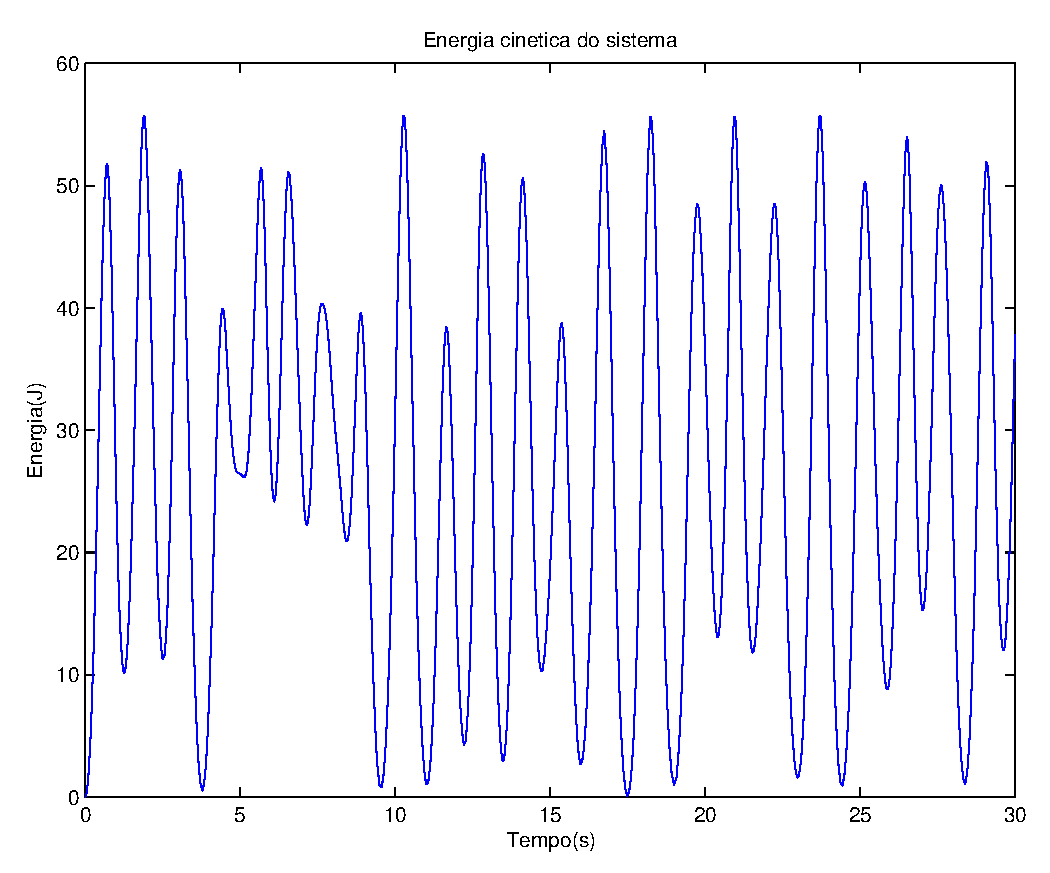
\includegraphics[width=0.8\linewidth]{../longsims/sime2kin.eps}
	\caption{Simulação 6 para energia do robô Puma sem atrito viscoso}
	\label{fig:energysim6nf}
\end{figure}

%TODO: revisar
Quando comparamos a simulação 5 com atrito (figuras \ref{fig:pumasim5} e \ref{fig:energysim5}) com a sem atrito (figuras \ref{fig:pumasim5nf} e \ref{fig:energysim5nf}) podemos notar que a primeira, sem oscilar muito, se acomoda em sua posição de equilíbrio estático (vertical com a ponta para baixo) após algum tempo, enquanto a segunda continua oscilando, com a junta $q_3$ dando mais voltas no sentido negativo que no positivo. Além disso, a energia da primeira se dissipa por meio do atrito conforme se observa na diminuição da amplitude dos picos sucessivos da energia cinética. Como na segunda não temos atrito, não podemos fazer a mesma observação. 

Observações semelhantes podem ser feitas comparando a simulação 6 com atrito (figuras \ref{fig:pumasim6} e \ref{fig:energysim6}) com a sem atrito (figuras \ref{fig:pumasim6nf} e \ref{fig:energysim6nf}).

Quando comparamos as duas simulações com atrito (figuras \ref{fig:pumasim5} e \ref{fig:energysim5} para a simulação 5 e figuras \ref{fig:pumasim6} e \ref{fig:energysim6} para a simulação 6) notamos que são muito semelhantes, pois partem de simulações com condições inicias próximas uma da outra. Quando comparamos as duas simulações sem atrito (figuras \ref{fig:pumasim5nf} e \ref{fig:energysim5nf} para a simulação 5 e figuras \ref{fig:pumasim6nf} e \ref{fig:energysim6nf} para a simulação 6), notamos também comportamentos semelhantes pelo mesmo motivo. Esse comportamento é diferente do encontrado na tese \cite{bb:tese}, mas devemos levar em consideração as diferenças entre o robô da tese e o puma560 e os erros numéricos da simulação, além da significância da posição inicial passada, embora tenhamos usados os mesmos ângulos para cada junta, esses ângulos implicam em uma configuração diferente para o robô. 


\subsection{Controle em malha fechada}
Para fazer um controle efetivo do robô, iremos agora considerar um controlador para o sistema em malha fechada. Ao fechar a malha, temos como entrada do controlador a diferença entre a referência e a saída, também chamada de erro. Conforme proposto na tese\cite{bb:tese} que estamos utilizando como base, iremos implementar um controlador PD, considerando cada uma das juntas como um sistema SISO.

Após verificar que os torques utilizados no robô Puma 560 eram aproximadamente um terço dos torques do robô utilizado na tese\cite{bb:tese}, utilizando como base os ganhos $K_p$ e $K_d$ do controlador calculado para o robô da tese, aprimoramos seus valores dividindo os da tese por três e chegamos em $K_p$ e $K_d$ dados pelas equações \ref{eq:kp} e \ref{eq:kd}.

\begin{equation}
\label{eq:kp}
K_p=\begin{bmatrix}
16.6667 & 0 & 0 & 0 & 0 & 0\\
0 & 16.6667 & 0 & 0 & 0 & 0\\
0 & 0 & 16.6667 & 0 & 0 & 0\\
0 & 0 & 0 & 16.6667 & 0 & 0\\
0 & 0 & 0 & 0 & 16.6667 & 0\\
0 & 0 & 0 & 0 & 0 & 20\\
\end{bmatrix}
\end{equation}
\begin{equation}
\label{eq:kd}
K_d=\begin{bmatrix}
6.6667 & 0 & 0 & 0 & 0 & 0\\
0 & 6.6667 & 0 & 0 & 0 & 0\\
0 & 0 & 6.6667 & 0 & 0 & 0\\
0 & 0 & 0 & 6.6667 & 0 & 0\\
0 & 0 & 0 & 0 & 6.6667 & 0\\
0 & 0 & 0 & 0 & 0 & 7.3333\\
\end{bmatrix}
\end{equation}

\subsubsection{Simulação 7}
Condições iniciais e referência:
\begin{equation}
\label{eq:sim7q}
q_{init}=\begin{bmatrix}
0 & 0 & 0 & 0 & 0 & 0
\end{bmatrix}^T
\end{equation}
\begin{equation}
\label{eq:sim7qd}
\dot{q_{init}}=\begin{bmatrix}
0 & 0 & 0 & 0 & 0 & 0
\end{bmatrix}^T
\end{equation}
\begin{equation}
\label{eq:sim7qr}
q_{ref}=\begin{bmatrix}
\frac{\pi}{2} & 0 & -\frac{\pi}{2} & \pi & \frac{\pi}{2} & -\pi
\end{bmatrix}^T
\end{equation}

\begin{figure}[H]
	\centering
	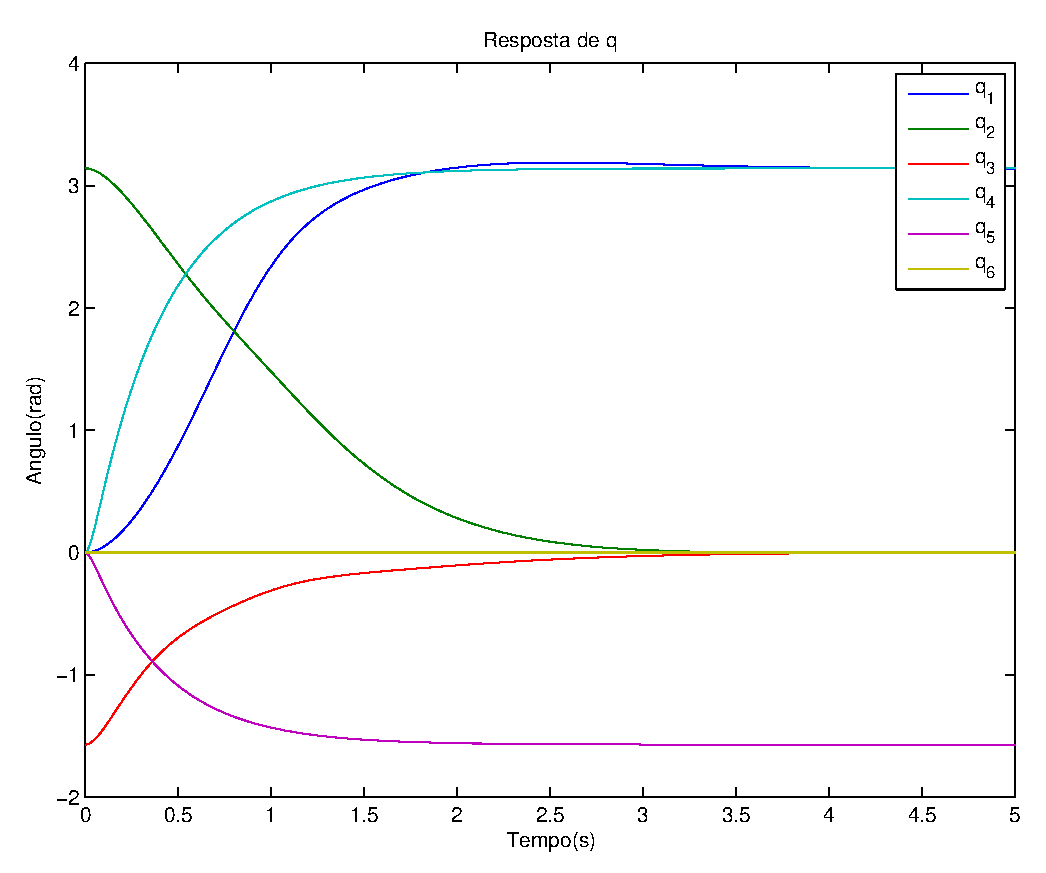
\includegraphics[width=0.8\linewidth]{../sim1cl}
	\caption{Simulação 7 para o robô Puma com controlador}
	\label{fig:pumasim7}
\end{figure}

\begin{figure}[H]
	\centering
	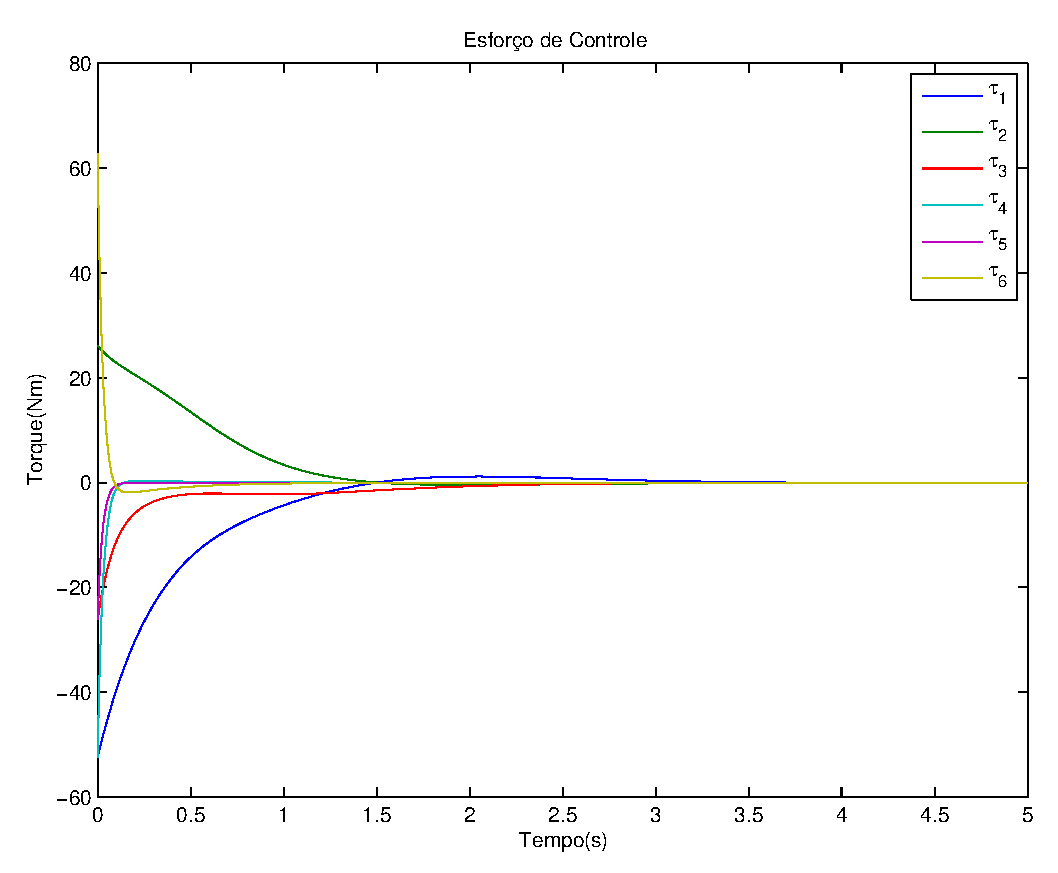
\includegraphics[width=0.8\linewidth]{../sim1clu}
	\caption{Esforços de controle para simulação 7 para o robô Puma com controlador}
	\label{fig:pumasim7clu}
\end{figure}

\subsubsection{Simulação 8}
Condições iniciais e referência:
\begin{equation}
\label{eq:sim8q}
q_{init}=\begin{bmatrix}
0 & \pi & -\frac{\pi}{2} & 0 & 0 & 0
\end{bmatrix}^T
\end{equation}
\begin{equation}
\label{eq:sim8qd}
\dot{q_{init}}=\begin{bmatrix}
0 & 0 & 0 & 0 & 0 & 0
\end{bmatrix}^T
\end{equation}
\begin{equation}
\label{eq:sim8qr}
q_{ref}=\begin{bmatrix}
\pi & 0 & 0 & \pi & -\frac{\pi}{2} & 0
\end{bmatrix}^T
\end{equation}

\begin{figure}[H]
	\centering
	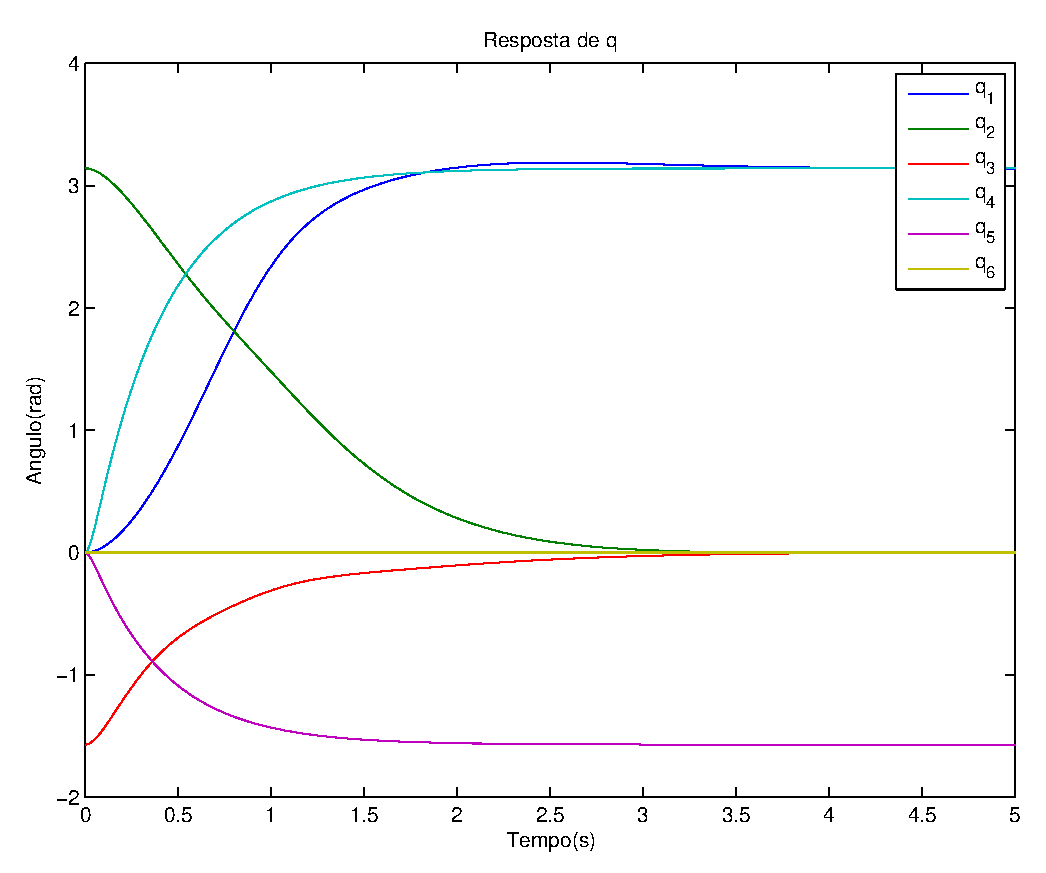
\includegraphics[width=0.8\linewidth]{../sim2cl}
	\caption{Simulação 8 para o robô Puma com controlador}
	\label{fig:pumasim8}
\end{figure}

\begin{figure}[H]
	\centering
	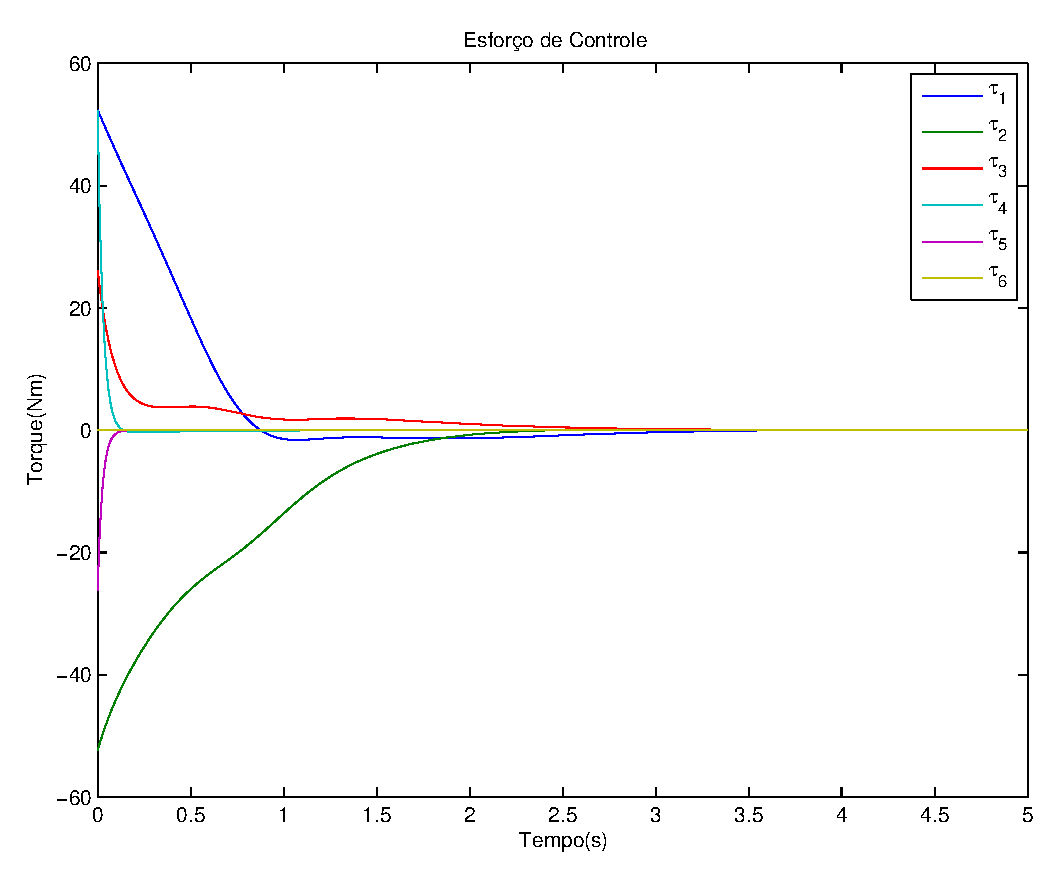
\includegraphics[width=0.8\linewidth]{../sim2clu}
	\caption{Esforços de controle para simulação 8 para o robô Puma com controlador}
	\label{fig:pumasim8clu}
\end{figure}

\subsubsection{Simulação 9}
Condições iniciais e referência:
\begin{equation}
\label{eq:sim9q}
q_{init}=\begin{bmatrix}
0 & \frac{\pi}{2} & -\frac{\pi}{2} & 0 & 0 & 0
\end{bmatrix}^T
\end{equation}
\begin{equation}
\label{eq:sim9qd}
\dot{q_{init}}=\begin{bmatrix}
0 & 0 & 0 & 0 & 0 & 0
\end{bmatrix}^T
\end{equation}
\begin{equation}
\label{eq:sim9qr}
q_{ref}=\begin{bmatrix}
-\pi & \pi & -\pi & -\pi & -\frac{\pi}{2} & \pi
\end{bmatrix}^T
\end{equation}

\begin{figure}[H]
	\centering
	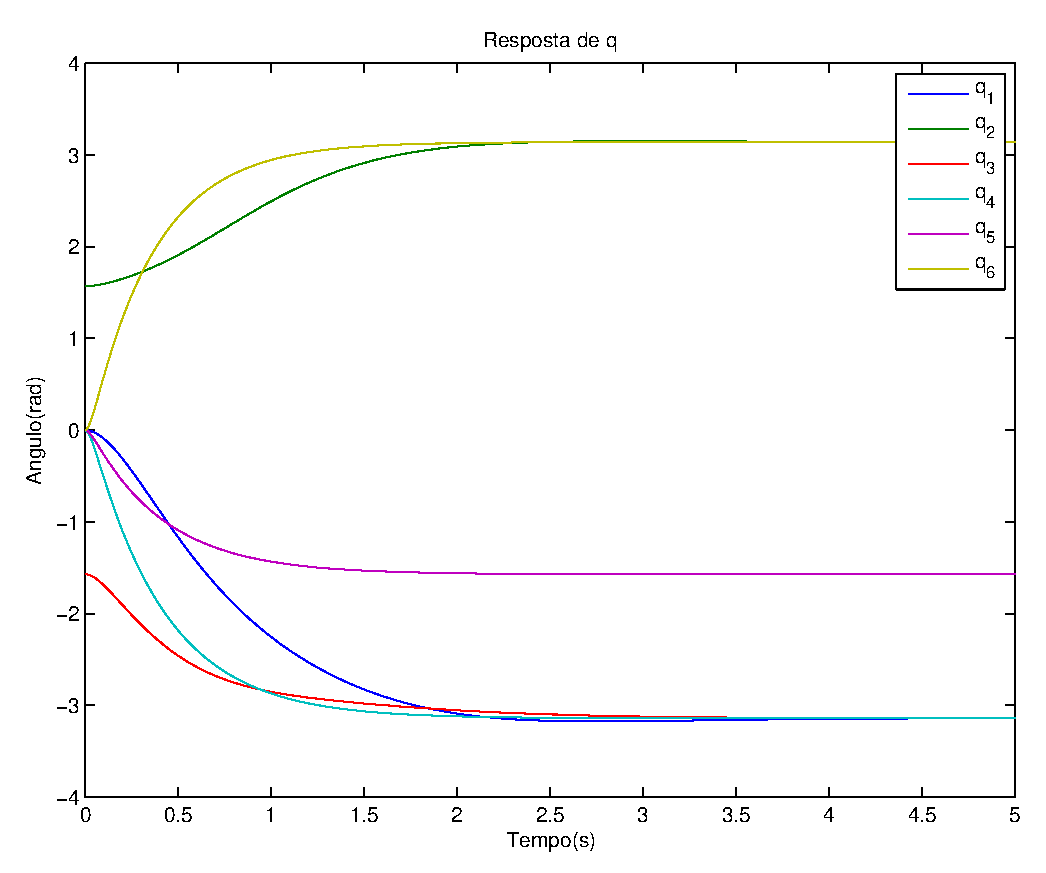
\includegraphics[width=0.8\linewidth]{../sim3cl}
	\caption{Simulação 9 para o robô Puma com controlador}
	\label{fig:pumasim9}
\end{figure}

\begin{figure}[H]
	\centering
	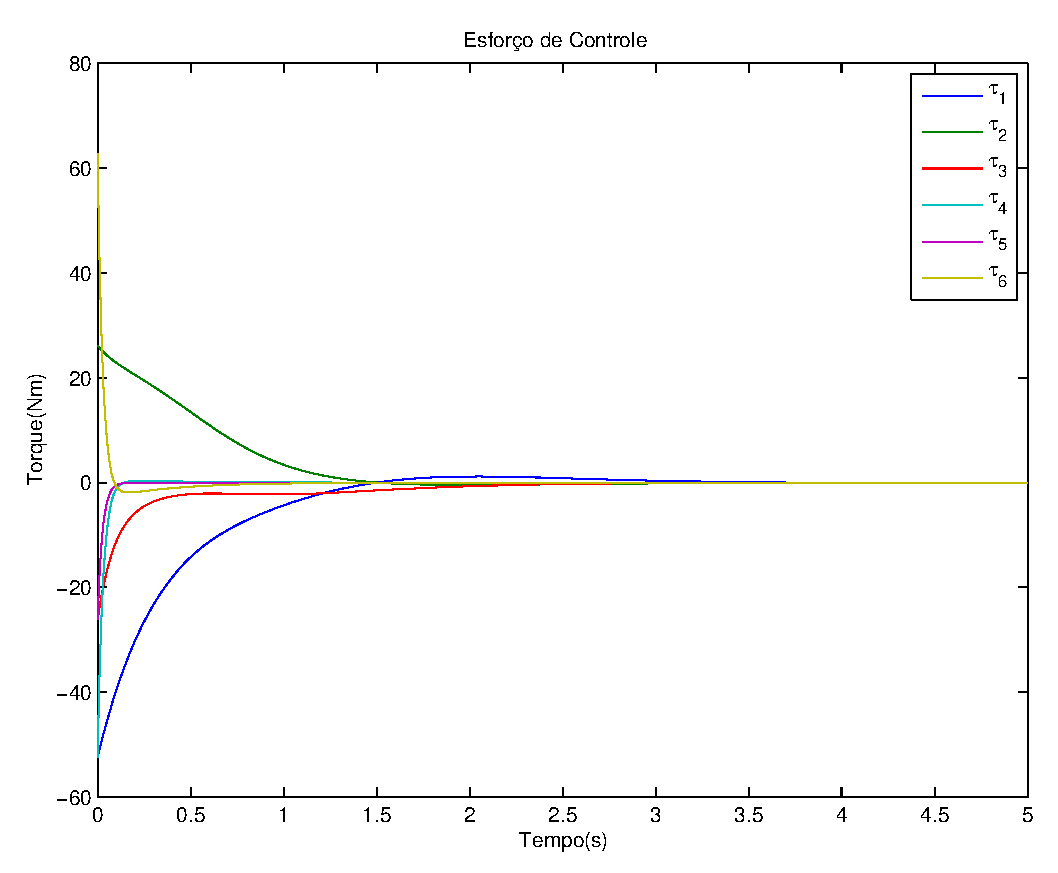
\includegraphics[width=0.8\linewidth]{../sim3clu}
	\caption{Esforços de controle para simulação 9 para o robô Puma com controlador}
	\label{fig:pumasim9clu}
\end{figure}

Observando as simulações nas figuras \ref{fig:pumasim7}, \ref{fig:pumasim8} e \ref{fig:pumasim9}, notamos que o robô é capaz de atingir a posição desejada em cada um dos casos, independentemente de suas condições iniciais de posição ou velocidade. Com ligação direta a este resultado, temos o esforço de controle de cada uma das juntas em cada uma das simulações representados nas figuras \ref{fig:pumasim7clu}, \ref{fig:pumasim8clu} e \ref{fig:pumasim9clu}.

No entanto, podemos notar também que os módulos desses esforços de controle são bastante elevados no início das simulações, para tentar levar o robô para a posição desejada o mais rápido possível, o que não é aplicável na realidade por limitações físicas dos atuadores no robô. Para obter uma simulação com características mais realistas, deve-se criar uma saturação nos esforços de controle de cada junta condizente com o modelo físico, assim o robô simulado terá seu comportamento mais próximo da realidade.

\section{Cinemática}
Para o estudo da cinemática, iremos usar o robô criado por ``ini\_Rbt"\cite{bb:inirbt}, e não o Puma 560 com que estávamos trabalhando até o momento. Foram feitos utilizando ``script" do Matlab em que descrevemos a trajetória espacial desejada, e o robô calcula os ângulos de suas juntas para cada ponto da trajetória por meio da cinemática inversa usando a toolbox\cite{bb:toolbox}. Estes valores são armazenados para criar a animação do movimento do robô, em que colocamos o robô em cada posição da sequência.

\subsection{Elipse}
Uma das trajetórias que testamos foi uma elipse no chão, e também uma elipse na parede, conforme figura \ref{fig:elipsec}. Notamos que os raios da elipse e sua distância em relação à base do robô possuem um limite, já que existe um alcance restrito ao robô dado pelo comprimento de seus elos.

\begin{figure}[H]
	\centering
	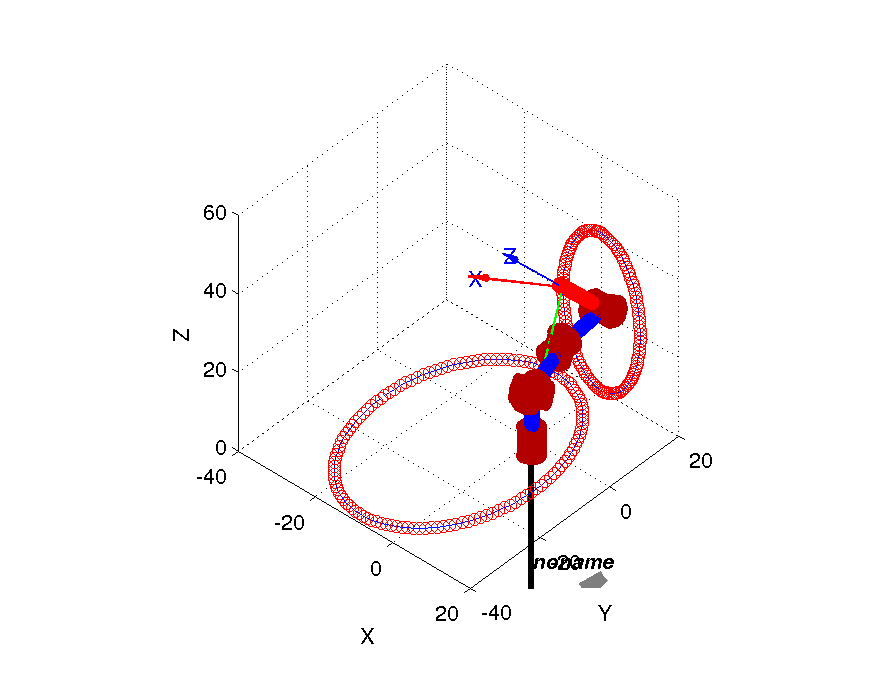
\includegraphics[width=0.8\linewidth]{../ellipses}
	\caption{Execução da trajetória em elipse no chão e na parede}
	\label{fig:elipsec}
\end{figure}


\section{Questões}
\begin{itemize}
	\item \textbf{Por que na seção ``Controle em malha fechada" os torques finais obtidos são nulos? O torque final não deveria ser igual ao torque de compensação da força da gravidade?}
	
	Conforme apontado por Herman Høifødt\cite{bb:tese} em sua tese, na seção 6.5.1, ao somar a carga gravitacional ao esforço de controle do controlador PD podemos controlar o sistema. Fizemos então a mesma simplificação que foi feita por ele na seção 6.5.2 de remover o termo gravitacional diretamente do modelo do robô ao invés de somar esse termo na resposta do controlador, por isso obtemos os torques finais como nulos.
	Se não nos utilizássemos dessa simplificação, a equação de nosso controlador seria da seguinte forma e o esforço final seria não nulo:
	
	\begin{equation}
		u = -K_p\cdot (q - q_r) -K_d\cdot\dot{q} + gravload(q);
	\end{equation}
	
	\item \textbf{Na seção ``Equilíbrio de energia cinética" foi indicado um comando do Matlab para se obter a matriz de massa/inércia no espaço das juntas $\rightarrow M(q)$. Como você faria para obter essa matriz de massa utilizando o método de Newton-Euler além de manipulação simbólica? Veja os apêndices B e C da tese\cite{bb:tese}. Essa matriz corresponde à matriz $M(q)$ da equação geral da dinâmica de um robô, como dado abaixo, onde ``u" é o vetor de torques nas juntas.}
	
	\begin{equation}
	\label{eq:mq}
	M(q)\ddot{q}+C(q,\dot{q})\dot{q}+g(q)=u
	\end{equation}
	
	Utilizando o método de Newton-Euler encontraríamos recursivamente, partindo da base para a ponta, a velocidade angular $\omega_i$ e a aceleração angular $\alpha_i$, representadas em relação à base, para cada um dos elos. Resolveríamos então, novamente de maneira recursiva, mas dessa vez da ponta para a base, o torque $\tau_i$, relacionado com as acelerações encontradas, chegando em fim em equações que nos dão o torque na junta i em função dos parâmetros $\ddot{q}$, $\dot{q}$, $q$ e $g$.
	\begin{equation}
		\tau_i(\ddot{q}, \dot{q}, q, g)
	\end{equation} 
	
	Isso pode ser feito da maneira detalhada na seção 3.2.2 da tese \cite{bb:tese}. Com essas equações, podemos determinar os termos da $m(q)_{i,j}$ da matriz $M(q)$ fazendo:
	\begin{equation}
		m(q)_{i,j} = \tau_i(x_j, 0, q, 0)
	\end{equation}
	Onde $x_j$ é o vetor unitário no qual todos os termos são 0 exceto o termo de índice j, que vale 1.
	
	\item \textbf{Por que essa matriz de massa $M(q)$ não é do tipo da matriz de massa abaixo de um corpo rígido, que é uma matriz $6x6$ com uma matriz diagonal $M$ e outra matriz de inércia do corpo J?}
	
	\begin{equation}
	\label{eq:m6x6}
	\bar{M}=\begin{bmatrix}
	M & 0\\
	0 & J
	\end{bmatrix}
	\end{equation}
	
	Essa matriz não corresponde à matriz de massa de um corpo rígido pois consideramos a transformação da base do robô para a garra do mesmo. Se olharmos as matrizes de transformação massa de um eixo $i$ em relação ao eixo $i-1$ veríamos que estas sim corresponderiam à matrizes de corpos rígidos, porém ao considerar o conjunto completo do robô não encontraremos um comportamento de corpo rígido, mas sim da junção de vários destes.
	
\end{itemize}

\begin{thebibliography}{widestlabel}
	\bibitem{bb:roteiro}{Roteiro do projeto disponibilizado para os alunos}
	\bibitem{bb:toolbox}{Peter Corke, Robotics Toolbox, disponível em http://www.petercorke.com/Robotics\_Toolbox.html}
	\bibitem{bb:inirbt}{Código ini\_Rbt.m fornecido pelo professor}
	\bibitem{bb:rbtsquare}{Código Rbtsquare.m fornecido pelo professor}
	\bibitem{bb:tese}{Herman Høifødt, Dynamic Modeling and Simulation of Robot Manipulators, The Newton-Euler Formulation, disponível em http://www.diva-portal.org/smash/get/diva2:436733/FULLTEXT01.pdf}
	
\end{thebibliography}
\end{document}

